\section{Anwendungsbeispiele}


\begin{frame}{Anwendungsbeispiele}
	Die Freifunkknoten kann man auf vielerlei Art und Weisen verwenden.
	Die Client-Ports verhalten sich hierbei wie ein großer Switch und die Batman Ports bieten eine Möglichkeit an
	beliebige Topologien zu bauen in denen dann vermittelt wird.
\end{frame}

\begin{frame}{kein Layer2 nach außen}
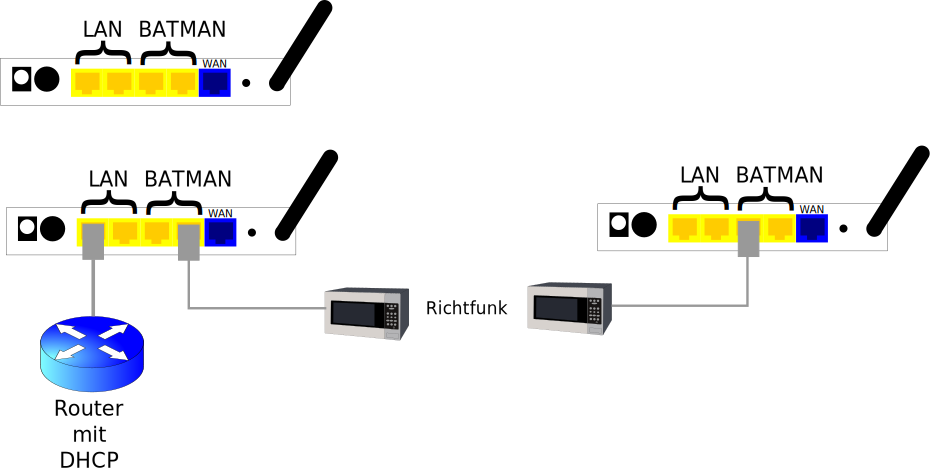
\includegraphics[width=0.9\textwidth]{img/svg/als_grosses_wlan.pdf}

Eine unabhängige Wolke kann ihr Netz von einem Router bekommen der einfach an einen der Client Ports angeschlossen wird.
Die Knoten können miteinander auch über spezielle Richtfunkstrecken verbunden werden.

\end{frame}


\begin{frame}{Standort mit mehreren Kanälen}
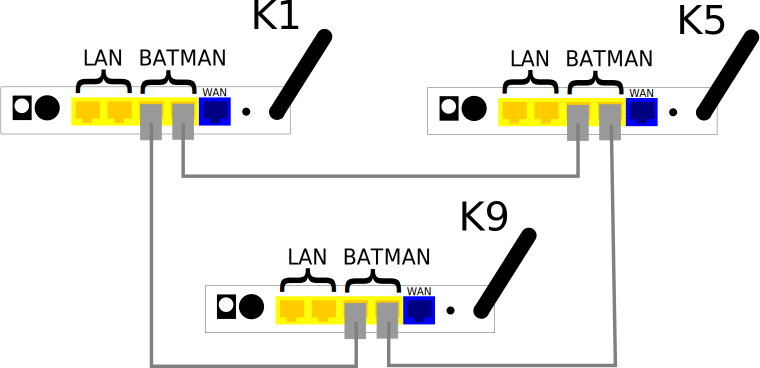
\includegraphics[width=0.5\textwidth]{img/svg/knoten_mit_mehr_kanaelen_richtungen.pdf}

Mehrere Knoten können beliebig untereinander per Kabel verbunden werden. Dies ermöglicht die Verwendung unterschiedlicher Funkkanäle oder Richtfunkantennen in unterschiedliche Richtungen.
\end{frame}

